\documentclass[a4paper,10pt]{article}
\usepackage[utf8]{inputenc}

\setlength\parindent{0pt}
\usepackage[english]{babel}
\usepackage[dvinames]{xcolor}
\usepackage[compact,small]{titlesec}
\usepackage{booktabs}
\usepackage{multirow}
\usepackage{amsfonts,amsmath,amssymb}
\usepackage{marginnote}
\usepackage[top=1.8cm, bottom=1.8cm, outer=1.8cm, inner=1.8cm, heightrounded, marginparwidth=2.5cm, marginparsep=0.5cm]{geometry}
\usepackage{enumitem}
\setlist{noitemsep,parsep=2pt}
\newcommand{\highlight}[1]{\textcolor{kuleuven}{#1}}
\usepackage{pythonhighlight}
\usepackage{cleveref}
\usepackage{graphicx}
\usepackage{algorithmic}
\usepackage{tabularx}

\newcommand{\nextyear}{\advance\year by 1 \the\year\advance\year by -1}
\newcommand{\thisyear}{\the\year}
\newcommand{\deadlineGroup}{November 27, \thisyear{} at 16:00 CET}
\newcommand{\deadlineCode}{December 18, \thisyear{} at 16:00 CET}
\newcommand{\deadlineReport}{January 4, \nextyear{} at 16:00 CET}

\newcommand{\ReplaceMe}[1]{{\color{blue}#1}}
\newcommand{\RemoveMe}[1]{{\color{purple}#1}}

\setlength{\parskip}{5pt}

%opening
\title{Artificial Neural Networks: Exercise session 1}
\author{Stijn Staring (r0620003)}

\begin{document}
\fontfamily{ppl}
\selectfont{}

\maketitle

%\section{\RemoveMe{Formal requirements}} \label{sec_this}

\section{Exercises of Section 2}
\textbf{Function approximation: comparison of various algorithms:
	Take the function $y = sin(x2) for x = 0 : 0:05 : 3$ and try to approximate it using a neural network with one hidden
	layer. Use different algorithms. How does gradient descent perform compared to other training algorithms?}\\

\textbf{Learing from target data without noise}\\
The neural network that is used in this section consists of one hidden layer with $ 50 $ hidden neurons and a single input and output neuron. The input data is a 1D array of x values. \\

%\textbf{Gradient descent vs Gradient descent with adaptive learning rate}\\
The gradient descent and the gradient descent with adaptive learning rate behave very similar for the first $ 15 $ iterations. Where they give both unsatisfactory results with a correlation coefficient between predictions and targets of only $ R = 0.08 $. Quality of the regression improves when $ 1000 $ epochs are performed. Here clearly the method of gradient descent with adaptive learning rate to update the weights performs better. The correlation coefficient of gradient descent with and without adaptive learning rate are respectively $ R = 0.535 $ and $ R = 0.857 $. All the results of the different methods to learn from noiseless data that further are discussed, are summarized by Table \ref{tab:corr_no_noise}.\\

It can be seen that all other methods behave equally bad as gradient descent when only $ 1 $ epoch is performed except for the Levenberg-Marquardt method. Already after one epoch is achieves a higher correlation between prediction and target values than both the gradient methods after $ 100 $ epochs. After $ 15 $ epochs it achieves as only method perfect linear correlation.\\ 

It should be noted that the disadvantage of the gradient descent method in comparison with other methods is that it has slow convergence in function of the amount of iterations in comparison with methods that are derivatives from the Newton method as for example the BFGS quasi Newton algorithm and Levenberg-Marquardt algorithm. One iteration of the later mentioned algorithms takes longer than one iteration of the Gradient descent. Using the amount of epochs as stopping criteria works therefore in the advantage of update methods that converge fast in function of the amount of iterations, but have iterations that are more calculation expensive. Therefore, it is expected that when a time limit is used as stopping criteria this will be in favour of the gradient descent method. \\

\begin{table}
	\centering
	\begin{tabular}{@{}l|lcr@{}} \toprule
		\textbf{Learning rule}    & $ 1 $ epoch & $ 15 $ epochs & $ 100 $ epochs \\\midrule
		\textbf{Gradient Descent}    & $ 0.0773 $  & $ -0.0818 $  & $ 0.575 $  \\
		\textbf{GD with adaptive learning rate} & $ 0.0773 $  & $ -0.0697 $  & $ 0.863 $  \\
		\textbf{Fletcher-Reeves} & $ 0.00198 $  & $ 0.790 $  & $ 0.999 $  \\
		\textbf{Polak-Ribier} & $ -0.0464 $  & $ 0.758 $  & $ 0.999 $  \\
		\textbf{BFGS} & $ -0.0625 $  & $ 0.857 $  & $ 1.00 $  \\
		\textbf{Levenberg-Marquardt} & $ 0.899 $  & $ 1.00 $  & $ 1.00 $  \\ \bottomrule
	\end{tabular}
	\caption{Correlation coefficients between predictions and targets of  different methods in function of the amount of epochs performed during training on noiseless data.}
	\label{tab:corr_no_noise}
\end{table}

%The performance of further methods with respect to the correlation coefficient is given in table \ref{tab:corr_no_noise} Using the ``Fletcher-Reeves'' conjugate gradient algorithm to update the weights decisevely outperforms a simple gradient descent in function of the amount of epochs. Already after $ 15 $ epochs a correlation coefficient of $ R = 0.736 $ is achieved and after $ 1000 $ epochs there is almost perfect regression with $ R = 0.99 $.\\

\textbf{Learing from target data without noise}\\
Now instead of performing a regression with a feedforward neural network on noiseless target data now additional noise is added by adding gaussian noise with a standard deviation of $ 0.2 $ and a mean of zero. The results of the neural network with respect to the correlation coefficient is shown in Table \ref{tab:corr_with_noise}.\\

It can be concluded that all methods perform also reasonably on data with noise. All methods behave only slightly worse when $ 100 $ epochs are performed.

\begin{table}
	\centering
	\begin{tabular}{@{}l|lcr@{}} \toprule
		\textbf{Learning rule}    & $ 1 $ epoch & $ 15 $ epochs & $ 100 $ epochs \\\midrule
		\textbf{Gradient Descent}    & $ -0.109 $  & $ -0.236 $  & $ 0.584 $  \\
		\textbf{GD with adaptive learning rate} & $ -0.109 $  & $ -0.212 $  & $ 0.807 $  \\
		\textbf{Fletcher-Reeves} & $ -0.153 $  & $ 0.602 $  & $ 0.982 $  \\
		\textbf{Polak-Ribier} & $ -0.0157 $  & $ 0.767 $  & $ 0.977 $  \\
		\textbf{BFGS} & $ -0.0725 $  & $ 0.900 $  & $ 0.974 $  \\
		\textbf{Levenberg-Marquardt} & $ 0.890 $  & $ 0.978 $  & $ 0.972 $  \\ \bottomrule
	\end{tabular}
	\caption{Correlation coefficients between predictions and targets of  different methods in function of the amount of epochs performed during training on data with added noise.}
	\label{tab:corr_with_noise}
\end{table}

\textbf{In this problem, the objective is to approximate a nonlinear function
	using a feedforward artificial neural network.}\\

\textbf{Define your datasets: your dataset consists now of X1;X2 and Tnew. Draw 3 (independent) samples of 1 000 	points each. Use them as the training set, validation set, and test set, respectively. Motivate the choice of the 	datasets. Plot the surface of your training set using the Matlab function scatteredInterpolant,plot3 	and mesh.}\\

Three datasets are developed respectively for training, validation and testing. The training data set is usually the largest and has as purpose to learn the weights of the network by making use of backpropagation algorithm to calculate the gradient and learning rules as discussed in Table \ref{tab:corr_no_noise} and Table \ref{tab:corr_with_noise}. The purpose of the validation to set the best suitable hyper parameters and tune design decisions of the neural network. A test set is used to determine the performance of the network on unseen data. Figure \ref{fig:surface} shows the surface that is the learning target of the training dataset. 

\begin{figure}[h!]
	\centering
	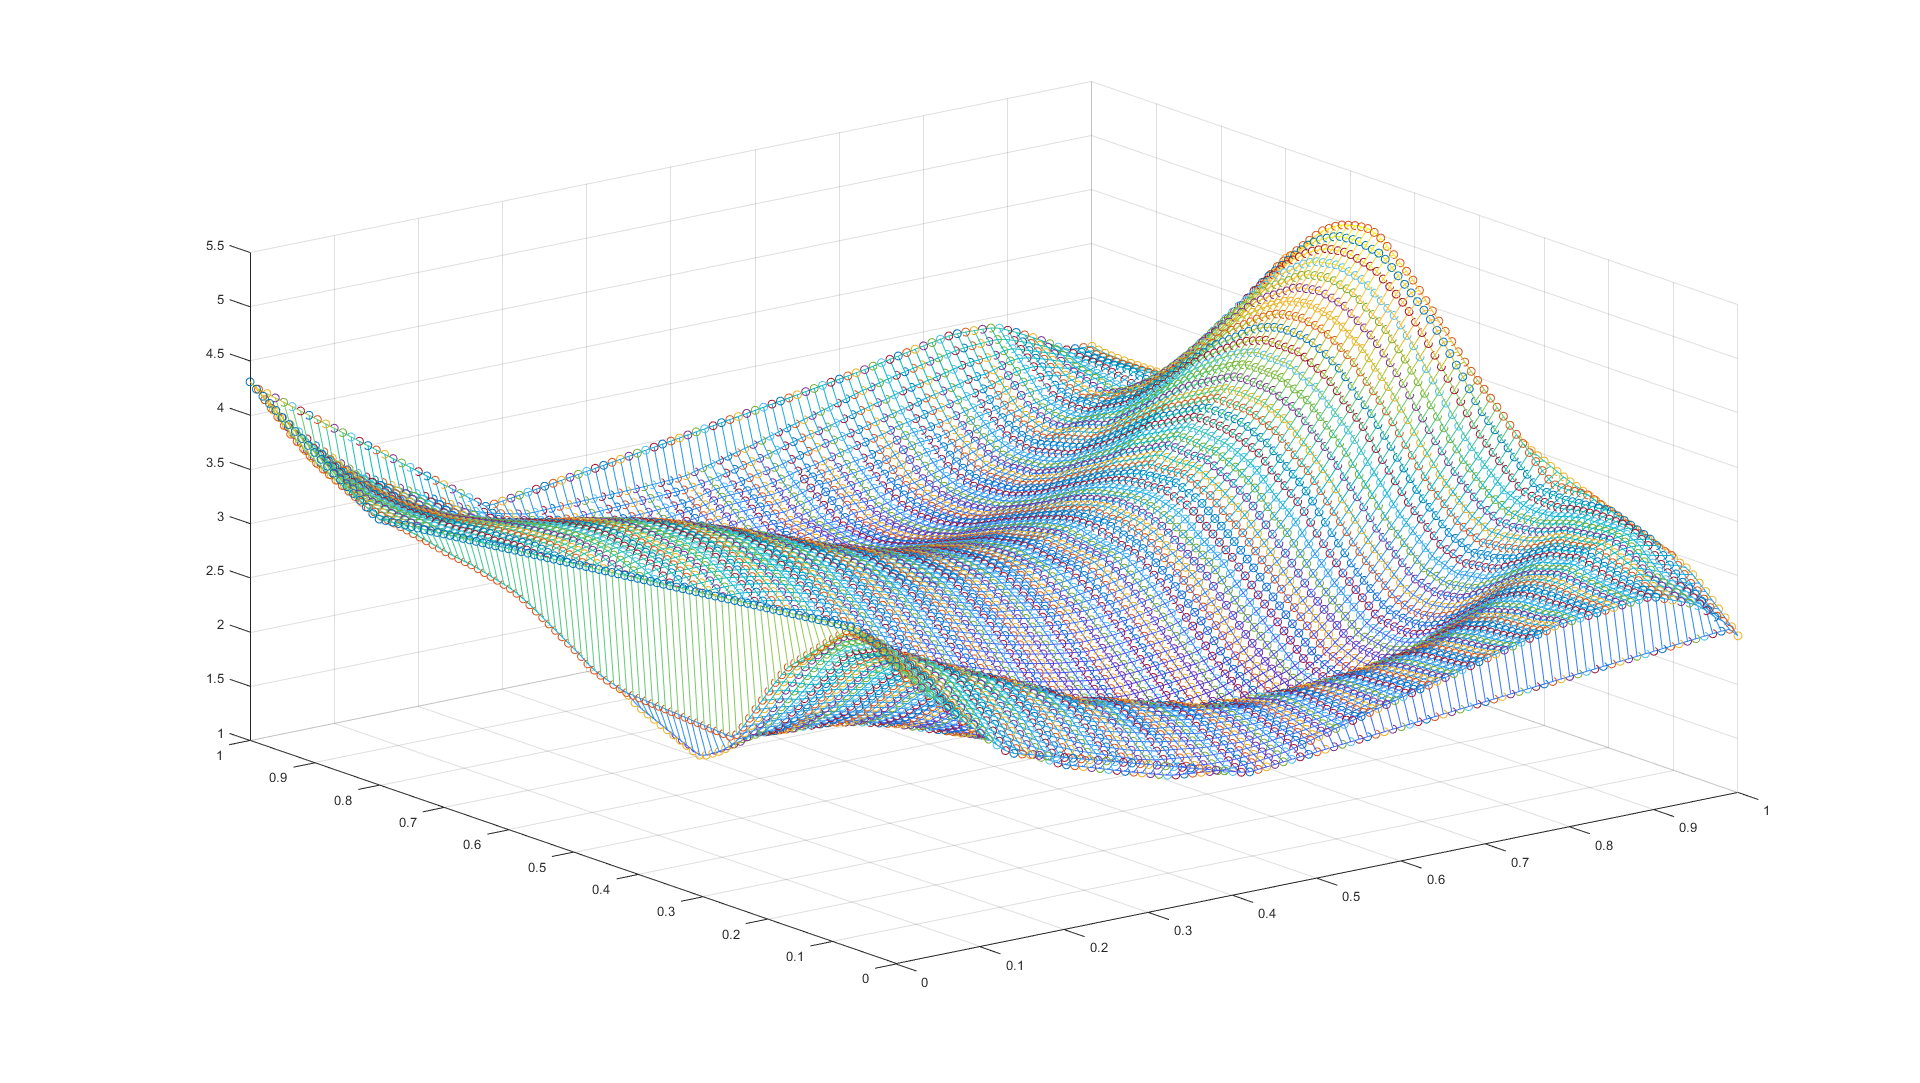
\includegraphics[width=1\textwidth]{surface.png}
	\caption{The visualization of the target surface of the training set.}
	\label{tab:surface}
\end{figure}


\textbf{Build and train your feedforward Neural Network: use the training and validation sets. Build the ANN with 2
	inputs and 1 output. Select a suitable model for the problem (number of hidden layers, number of neurons in
	each hidden layer). Select the learning algorithm and the transfer function that may work best for this problem.
	Motivate your decisions. When you try different networks, clearly say at the end which one you would select as
	the best for this problem and why.}\\

The feedforward neural network is build by using the Deep Learning Toolbox in Matlab. Table \ref{tab:design} shows an overview of design decisions that have been tried. Each combination is run $ 10 $ times from which the average mean square error is calculated. In order to deal with overfitting the validation set is used to perform early stopping. This means that during training the error on the validation set may only $ 10 $ increase directly after each other. If this amount is exceeded the learning is stopped. Additionally, to avoid overfitting a regulation term is added in the objective function during training. This regulation term L2 norm of the weights and a regulation parameter is used to determine the importance of the regulation term in comparison with the training error on the targets.\\ The training is stopped when the max amount of $ 500 $ iterations is reached, the training error becomes smaller then $ 10^-3 $ or when the learning takes longer then $ 1 $ minute. The activation functions that are used are the default ones of the Matlab toolbox. For a hidden layer and the output layer are respectively the ``tansig'' and ``purelin'' functions used.\\
It was found after similations that the  


%\begin{table}
%	\centering
%	\begin{tabular}{@{}ccr@{}} \toprule
%		\textbf{Design Variable}    & Option \midrule
%		Regulation parameter & $ 0.890 $  \\ \bottomrule
%	\end{tabular}
%	\caption{Correlation coefficients between predictions and targets of  different methods in function of the amount of epochs performed during training on data with added noise.}
%	\label{tab:corr_with_noise}
%\end{table}









\textbf{Performance Assessment: evaluate the performance of your selected network on the test set. Plot the surface of
	the test set and the approximation given by the network. Plot the error level curves. Compute the Mean Squared
	Error on the test set. Comment on the results and compare with the training performance. What else could you
	do to improve the performance of your network?}\\

When a validation set is given the Matlab toolbox takes by default the Matlab software applies early stopping to deal with overfitting.

the Tansig activation function is used in the hidden layers. 

The output layer uses the Purelin activation function. 

Looking at the performance by taking the average of $ 5 $ iterations

In the assessment of the amount of hidden neurons, only tested each layer with an equal amount of hidden layers. 


The best configuration of the neural networks is based on the best MSE performance on the validation set. 

Using $ 1000 $ epochs. 

Every training session of a neural network is given a time budget of $ 1 min $

\section{Exercises of Section 5}

\subsection{Main improvements} 

%\begin{figure}[h!]
%	\centering
%	\includegraphics[width=1.0\textwidth]{RNN.png}
%	\caption{Figure of the logical flow of a vanilla RNN with a hidden state (source \cite{Czum2020}).}
%	\label{fig:RNN}
%\end{figure}

%\begin{table}
%  \centering
%  \begin{tabular}{@{}llr@{}} \toprule
%    \multicolumn{2}{c}{Item} \\ \cmidrule(r){1-2}
%    Animal    & Description & Price (\$)\\ \midrule
%    Gnat      & per gram    & 13.65 \\
%              & each        & 0.01 \\
%    Gnu       & stuffed     & 92.50 \\
%    Emu       & stuffed     & 33.33 \\
%    Armadillo & frozen      & 8.99 \\ \bottomrule
%  \end{tabular}
%  \caption{A table with the correct layout.}
%  \label{tab:ok}
%\end{table}


%\cite{fast_alg}
%\cite{inver_over}

\bibliographystyle{abbrv}
%\bibliography{ANN1}

\end{document}
